\section{Additional Experiments}

\subsection{Controlled Synthetic Mechanism Checks}
\label{app:controlled-synthetic}

The controlled experiments in the main text are designed to isolate the role
of the scalar link. Table~\ref{tab:linear-consistency-controlled} first checks
a negative control: when the source is linear Tucker, NTD-PL does not improve
by inventing nonlinear terms. The only exception is an affine offset, where
the constant link term is the intended correction.

\begin{table}[ht]
  \centering
  \caption{Linear consistency on synthetic Tucker tensors. In the linear
  negative control, effective \(p>1\) contributions remain small except for
  the intended affine offset case.}
  \label{tab:linear-consistency-controlled}
  {\small
  \setlength{\tabcolsep}{4.5pt}
  \renewcommand{\arraystretch}{1.06}
  \begin{tabular}{@{}l ccc ccc@{}}
\toprule
\multirow{2}{*}{Method} &
\multicolumn{3}{c}{bias \(=0\)} &
\multicolumn{3}{c}{bias \(=0.5\)} \\
\cmidrule(lr){2-4}\cmidrule(l){5-7}
& RMSE$\downarrow$ & NMSE(dB)$\downarrow$ & \(p>1\) &
  RMSE$\downarrow$ & NMSE(dB)$\downarrow$ & \(p>1\) \\
\midrule
Tucker & \textbf{0.0114} & \textbf{-38.88} & -- &
0.0647 & -24.05 & -- \\
NTD-PL, \(\beta_0=0\) & 0.0116 & -38.72 & 4.19\% &
0.0522 & -25.85 & 39.17\% \\
NTD-PL, \(\beta_0\) free & 0.0117 & -38.65 & 3.19\% &
\textbf{0.0118} & \textbf{-38.58} & 2.98\% \\
\bottomrule
\end{tabular}

  }
\end{table}

For the nonlinear controlled tensors, the nonlinearity is introduced as an
orthogonal residual rather than by directly setting \(Y=g(S^\star)\). Let
\(S^\star\) be the linear low-rank Tucker backbone and let \(g\) be one of the
candidate scalar responses. We form
\begin{equation}
  R^\star
  =
  g(S^\star)
  -
  \frac{\langle g(S^\star),S^\star\rangle}{\|S^\star\|_F^2}\,S^\star,
  \label{eq:controlled-orthogonal-residual}
\end{equation}
and, when \(\|R^\star\|_F>0\), normalize it as
\begin{equation}
  \widetilde R^\star
  =
  \frac{\|S^\star\|_F}{\|R^\star\|_F}R^\star .
  \label{eq:controlled-normalized-residual}
\end{equation}
The observed tensor is then
\begin{equation}
  Y_\alpha
  =
  \sqrt{1-\alpha}\,S^\star
  +
  \sqrt{\alpha}\,\widetilde R^\star,
  \qquad 0\le \alpha\le 1 .
  \label{eq:controlled-residual-mixture}
\end{equation}
By construction, \(\langle S^\star,\widetilde R^\star\rangle=0\) and
\(\|\widetilde R^\star\|_F=\|S^\star\|_F\), so \(\alpha\) is exactly the
energy fraction assigned to the nonlinear residual. This keeps the total
energy fixed while moving the observation away from the linear Tucker
backbone. The candidate residual families are \(g(s)=s^2+s^3\),
\(g(s)=(\exp(\kappa s)-1)/\kappa\), and \(g(s)=\tanh(\kappa s)\),
with \(\kappa\) set from the input range.

The main text reports the nonlinear alpha sweep and degree sweep.
Figure~\ref{fig:controlled-training-curves} shows that degree continuation
activates higher powers with systematic loss drops at relevant degrees.
Table~\ref{tab:controlled-beta-contribution} complements those figures with a
small but consistent term-mass concentration effect: the dominant contribution
usually lands on the degree that matches the injected response, while smooth
odd links spread mass across nearby odd orders.

\begin{figure}[ht]
  \centering
  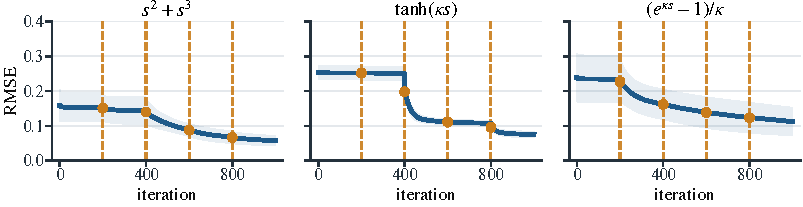
\includegraphics[width=0.98\linewidth]{figures/controlled_nonlinear_step_strip.pdf}
  \caption{NTD-PL training curves for controlled nonlinear mechanism checks at
  \(\alpha=0.25\) and \(P=5\). Dashed vertical lines mark degree activations,
  which produce systematic drops when the activated degree matches the
  response structure.}
  \label{fig:controlled-training-curves}
\end{figure}

\begin{table}[ht]
  \centering
  \caption{Effective NTD-PL term contributions under moderate nonlinearity,
  reported as percentages over ten seeds. Polynomial targets concentrate mass
  at matching nonlinear degrees, while odd smooth links place most nonlinear
  mass on odd powers.}
  \label{tab:controlled-beta-contribution}
  {\small
  \setlength{\tabcolsep}{4pt}
  \renewcommand{\arraystretch}{1.08}
  \begin{tabular}{@{}l*{7}{c}@{}}
\toprule
Link & \multicolumn{7}{c}{Effective contribution (\%)} \\
\cmidrule(lr){2-8}
 & $p=0$ & $p=1$ & $p=2$ & $p=3$ & $p=4$ & $p=5$ & $p=6$ \\
\midrule
\(s^2\) & 0.5 & 43.3 & \textbf{23.2} & 5.8 & 8.2 & 9.1 & 9.8 \\
\(s^2+s^3\) & 0.1 & 24.1 & 9.8 & \textbf{38.1} & 7.3 & 11.5 & 9.1 \\
\(\sin(\kappa s)\) & 0.1 & 37.7 & 0.6 & \textbf{35.4} & 2.8 & 19.8 & 3.6 \\
\(\tanh(\kappa s)\) & 0.2 & 37.9 & 1.3 & \textbf{30.9} & 5.4 & 17.3 & 7.0 \\
\bottomrule
\end{tabular}

  }
\end{table}

\subsection{CAVE Completion Significance and Robustness}
\label{app:single-rank-completion}

The main text reports the full-resolution random-missing CAVE completion table
at rank \((33,33,4)\). We do not repeat that table here; instead,
Table~\ref{tab:cave-completion-significance} gives the paired sign and
Wilcoxon tests for the same protocol.

\begin{table}[ht]
  \centering
  \caption{Paired significance tests for full-resolution CAVE completion at
  rank \((33,33,4)\). Metrics are computed only on missing entries.}
  \label{tab:cave-completion-significance}
  \scriptsize
  \resizebox{\linewidth}{!}{\begin{tabular}{@{}c*{4}{c}*{4}{c}@{}}
\toprule
 & \multicolumn{4}{c}{RMSE} & \multicolumn{4}{c}{SAM} \\
\cmidrule(lr){2-5}\cmidrule(l){6-9}
$\rho$ & W/L & Med. gain & Sign $p$ & Wilcoxon $p$ & W/L & Med. gain & Sign $p$ & Wilcoxon $p$ \\
\midrule
0.1 & 14/1 & 0.0027 & 9.77$\times 10^{-4}$ & 1.22$\times 10^{-4}$ & 14/1 & 2.9742 & 9.77$\times 10^{-4}$ & 8.54$\times 10^{-4}$ \\
0.3 & 14/1 & 0.0027 & 9.77$\times 10^{-4}$ & 1.22$\times 10^{-4}$ & 13/2 & 1.9194 & 0.007 & 0.004 \\
0.5 & 14/1 & 0.0026 & 9.77$\times 10^{-4}$ & 1.22$\times 10^{-4}$ & 13/2 & 1.6566 & 0.007 & 0.012 \\
0.7 & 14/1 & 0.0027 & 9.77$\times 10^{-4}$ & 1.22$\times 10^{-4}$ & 12/3 & 1.3394 & 0.035 & 0.048 \\
\bottomrule
\end{tabular}
}
\end{table}

\subsection{Link Refresh Residual Diagnostic}
\label{app:posthoc-calibration-baselines}

The diagnostic used in the main text reuses the Link Refresh step from
Section~\ref{sec:optimization} as a one-round residual probe. Let
\(\widehat{\cY}_{\mathrm{T}}\) denote the Tucker output and \(\cY\) the target
tensor. Starting from this fitted Tucker latent tensor, we update only the
scalar polynomial coefficients by fitting
\[
  h_{\gamma}(x)=\sum_{p=0}^{4}\gamma_p x^p
\]
by ridge regression on pairs
\((\widehat Y_{\mathrm{T},\mathbf i},Y_{\mathbf i})\). In full reconstruction,
all entries are used for this fit. In completion, the fit uses only observed
entries and is then evaluated on held-out entries. The fitted map is applied
entrywise to \(\widehat{\cY}_{\mathrm{T}}\). We summarize this cheap refresh by
the Link Refresh diagnostic
\[
  D_{\mathrm{link}}
  =10\log_{10}\!\left(
  \frac{\|\cY_{\mathrm{eval}}-\widehat{\cY}_{\mathrm{T}}\|_F^2}
  {\|\cY_{\mathrm{eval}}-\widehat{\cY}_{\mathrm{link}}\|_F^2}
  \right),
\]
which measures, on a log scale, how much Tucker residual energy is removed on
the task-specific evaluation entries. In other words, it measures how much
shared scalar-link yield is already present before the full NTD-PL alternating
solver starts reshaping the Tucker parameters.

\subsection{CAVE Completion Scene Diagnostics}
\label{app:cave-completion-scene-diagnostics}

Figure~\ref{fig:cave-link-yield-scatter-appendix} supplements the main CAVE
diagnostic table with the scene-level scatter plots used to visualize the link
yield across missing rates. The plots show the same diagnostic relationship
between \(D_{\mathrm{link}}\) and held-out RMSE$^\ast$ gain, now at the scene
level.

\begin{figure}[ht]
  \centering
  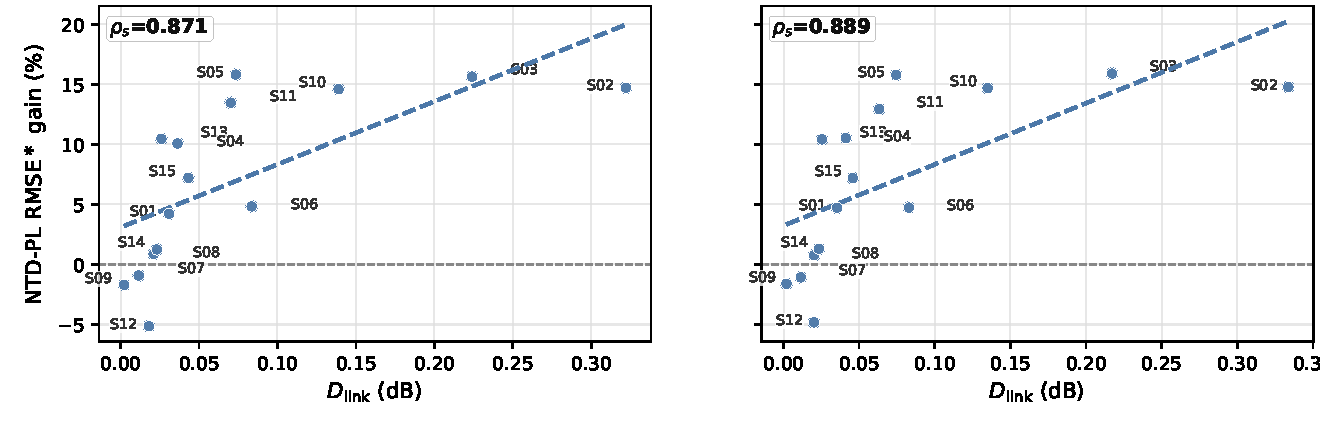
\includegraphics[width=0.95\linewidth]{figures/cave_link_yield_scatter.pdf}
  \caption{Scene-level supplement for the CAVE completion diagnostic table.
  The left and right panels use missing rates 0.3 and 0.5, respectively;
  \(D_{\mathrm{link}}\) from frozen-backbone Link Refresh predicts larger
  held-out RMSE$^\ast$ gains.}
  \label{fig:cave-link-yield-scatter-appendix}
\end{figure}

\subsection{Non-HSI Link Refresh Diagnostics}
\label{app:nonhsi-link-diagnostics}

\begin{table}[ht]
  \centering
  \caption{Dataset-level statistics behind the non-HSI diagnostic scatter in
  Figure~\ref{fig:nonhsi-link-scatter}. The gain columns report mean NTD-PL
  RMSE improvement over independently fitted matched-rank Tucker within
  \(D_{\mathrm{link}}\) terciles.}
  \label{tab:nonhsi-link-diagnostic-stats}
  \small
  \renewcommand{\arraystretch}{1.08}
  \setlength{\tabcolsep}{4.2pt}
  \begin{tabular*}{\linewidth}{@{\extracolsep{\fill}}llrrrrrr@{}}
  \toprule
  Domain & Dataset & Units & Med. \(D_{\mathrm{link}}\) &
  \(\rho_s\) & Low & Mid & High \\
  \midrule
  Natural images & CBSD68 & 68 & 0.091 & 0.85 & 4.17\% & 8.40\% & 14.60\% \\
  Natural images & CIFAR-10 & 1000 & 0.008 & 0.93 & -0.01\% & 2.59\% & 7.85\% \\
  Object-view & COIL-100 & 100 & 0.208 & 0.93 & 2.77\% & 5.46\% & 9.14\% \\
  Object-view & smallNORB & 25 & 0.264 & 0.95 & 6.92\% & 9.91\% & 14.16\% \\
  Action video & KTH-Action & 240 & 0.107 & 0.88 & 2.74\% & 4.27\% & 10.87\% \\
  Action video & UCF101 & 240 & 0.065 & 0.89 & 1.44\% & 2.97\% & 5.89\% \\
  \bottomrule
  \end{tabular*}
\end{table}

The main diagnostic figure uses per-unit non-HSI experiments rather than
collection-level tensors. CBSD68 \citep{martin2001database}
uses per-image units resized to \(96\times96\times3\) with rank
\((32,32,3)\). CIFAR-10
\citep{krizhevsky2009learning} uses 1000 class-balanced test images of shape
\(32\times32\times3\) with rank \((20,20,3)\). COIL-100
\citep{nene1996coil100} uses one object at a time as a
\(36\times48\times48\times3\) view tensor with rank \((8,12,12,2)\).
smallNORB \citep{LeCun2004SmallNORB} uses one object instance at a time as an
\(18\times64\times64\times2\) stereo view tensor with rank
\((12,24,24,2)\). KTH-Action \citep{Schuldt2004KTHActions} and UCF101
\citep{Soomro2012UCF101} provide the action-video tensor units used in the
main diagnostic scatter. All units are max-normalized independently, and
diagnostic labels are assigned only from \(D_{\mathrm{link}}\), not from NTD-PL
gain.

\paragraph{Compute resources.}
\label{app:compute-resources}
The reported runs used a CPU Python implementation based on NumPy, SciPy, and
TensorLy on a workstation with a 13th Gen Intel Core i5-13400F CPU
(10 physical cores, 16 logical workers), 32 GB system RAM, Windows 11, and
Python 3.13. An NVIDIA RTX 5060 GPU with 8 GB memory was present, but the
reported scripts do not use GPU kernels and do not require GPU memory. Sweep
scripts cap BLAS/OpenMP threads per worker and parallelize independent jobs,
using up to 12 workers for the main low-rank sweeps and 6 workers for the
diagnostic batches. From the recorded runtime fields, controlled synthetic
residual jobs were sub-second to about 1 s per configuration. Full-resolution
CAVE reconstruction took about 10--17 s per scene for matched-rank Tucker and
172--217 s per scene for NTD-PL in the main low-rank reconstruction sweep.
CAVE random completion runs took about 0.9--18.6 s per scene/mask/seed
(3.3--18.6 s for NTD-PL), while structured completion runs were about
1.6--5.0 s. The frozen-backbone CAVE Link Refresh diagnostic itself took about
0.12--0.59 s per fitted refresh; the associated full NTD-PL completion fits
used for comparison were on the order of 168--258 s in the recorded diagnostic
runs. Non-HSI diagnostic batches were run with 6 CPU workers: the
CBSD68/CIFAR-10/COIL-100/smallNORB batch took about 77 s wall-clock, and the
KTH-Action and UCF101 video batches took about 5--6 minutes each. Per-unit
NTD-PL runtimes in those diagnostics ranged from about 0.07--0.28 s for image
units, 1.2--2.7 s for object-view units, and 6.3--9.8 s for action-video
units. Peak memory was not instrumented per run; empirically the largest
reported CPU runs completed within the 32 GB system RAM budget.

\subsection{Dataset Asset and Usage Information}
\label{app:dataset-assets}

All datasets used in the experiments are public research benchmarks. We use
them only for reconstruction, completion, or diagnostic evaluation, and the
anonymous supplement redistributes processed summaries and scripts rather than
raw dataset files.

\begin{table}[ht]
  \centering
  \caption{Dataset sources and usage notes. ``No'' in the redistribution
  column means that raw data files are not included in the supplement.}
  \label{tab:dataset-asset-usage}
  \scriptsize
  \renewcommand{\arraystretch}{1.10}
  \setlength{\tabcolsep}{3pt}
  \begin{tabularx}{\linewidth}{@{}p{0.15\linewidth}p{0.25\linewidth}Xp{0.17\linewidth}@{}}
  \toprule
  Dataset & Source / citation & License or usage note & Redistribution / use \\
  \midrule
  CAVE Multispectral Image Database &
  Columbia CAVE Laboratory repository; \citep{cave_multispectral_database,yasuma2010gapc} &
  Official page provides public download and citation information, but does not
  specify a standard license in the page metadata available to us. Used only for
  research evaluation. &
  No; CAVE reconstruction, completion, and Link Refresh diagnostics. \\
  CBSD68 / Berkeley natural images &
  Berkeley Segmentation Dataset page; \citep{martin2001database} &
  Official BSDS usage statement permits use for research and non-commercial
  purposes only and requests citation of the Berkeley dataset. &
  No; non-HSI diagnostic evaluation. \\
  CIFAR-10 &
  University of Toronto CIFAR page; \citep{krizhevsky2009learning} &
  Official page provides public research benchmark downloads and citation, but
  does not specify a standard license in the page metadata available to us. &
  No; non-HSI diagnostic evaluation. \\
  COIL-100 &
  Columbia Object Image Library page; \citep{nene1996coil100} &
  Official page provides public download and citation information, but does not
  specify a standard license in the page metadata available to us. Used only for
  research evaluation. &
  No; non-HSI diagnostic evaluation. \\
  smallNORB &
  NYU/Yann LeCun dataset page; \citep{LeCun2004SmallNORB} &
  Official page states that the database is provided for research purposes,
  cannot be sold, and should be cited when used in publications. &
  No; non-HSI diagnostic evaluation. \\
  KTH-Action &
  KTH action-recognition dataset page; \citep{Schuldt2004KTHActions} &
  Official page states that the database is publicly available for
  non-commercial use and requests citation of the ICPR 2004 paper. &
  No; non-HSI diagnostic evaluation. \\
  UCF101 &
  UCF CRCV dataset page; \citep{Soomro2012UCF101} &
  Official page provides public benchmark downloads and citation, but does not
  specify a standard license in the page metadata available to us. Used only for
  research evaluation. &
  No; non-HSI diagnostic evaluation. \\
  \bottomrule
  \end{tabularx}
\end{table}
